%----------------------------------------
% Write your notes here
%----------------------------------------

\section{Regression and Model Evaluation} 
    Regression is a statistical analysis procedure that can
summarize the current data, predict future outcomes and describe the associations between the predictors and the outcomes. In today's class, we used the file from last lecture with information on 225,000 anonymous Nielsen panelists, containing their age, gender, and the number of pages (~distinct urls) they typically access on their web browser each day, filtering out users with zero pageviews.


\subsection{Plotting predicted vs. actual values}

We fit the predicted and actual values based on the model and differentiate them with respect to their gender. Each dot on the plot corresponding to an 'age' value is computed by taking the median of all page views in that age. The size of the dots is proportional to the number of people with that age. We aim to find the best fit for data by visual interpretation.

\begin{itemize}
  \item Too many features makes it difficult to understand the plot.so we first start by plotting the predicted vs.actual values along with a diagonal line to indicate how a perfect model would fit. The points are binned such that each dot represents the average actual outcomes of all the observations that were predicted to be in a small range.
  \item  We then differentiate the data based on gender. We can notice that both the actual and predicted outcomes are higher in female on average.
  \item We can also choose to differentiate with respect to a continuous attribute such as age.
\end{itemize}

\subsection{Model Variability}
Until now, the model seems to do a good job. However, once the binning is removed and all the 225,000 points are plotted, we can notice much variation within the individual observations. The variance between the output is greater than the individual variance as shown in the figure below. Thus, viewing the average data is not same as viewing the entire data. \\

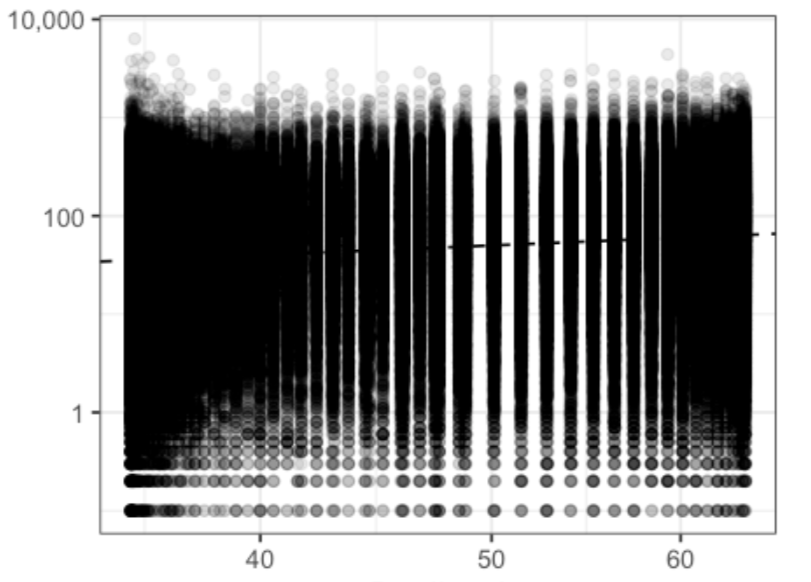
\includegraphics[width=0.5\textwidth]{figures/var.PNG}

\subsection{Quantifying the model}
Now, it is evident that variance is an important information about the data.We need to account for variation of the data along with the trend or correlation in the data.

One useful metric of evaluation is the RMSE (Root Mean Square Error). It represents the standard deviation between the differences of predicted value and average value, given as,
\begin{equation}
    RMSE = \sqrt{\frac{1}{N}\sum_{i=1}^{N}(y_i - \hat{y})^2}
\end{equation}

we have,
\begin{equation}
    MSE_{\text{baseline}} = \frac{1}{N}\sum_{i=1}^{N}(y_i - \hat{y})^2
\end{equation}

Thus, we define $R^2$, the fraction of variance explained, as,
\begin{equation}
    R^2 = \frac{MSE_{\text{baseline}} - MSE_{\text{model}}}{MSE_{\text{baseline}}}
\end{equation}

For the previous plot, the RMSE is very high with a value of about 165. This implies that the prediction model is almost same as randomly guessing the outcome.

\section{Overfitting}

A sufficiently complex model can fit any data and attain almost zero error on the data. However, it should be noted that the models should be complex enough to explain the past but simple enough to generalize to the future. 
This can be achieved by splitting the data into 3 sets.
\begin{itemize}
  \item Training dataset - The model is trained using this data
  \item Validation dataset -  This dataset is used to test the performance of the model/classifier.
  \item Testing dataset -  The dataset gives an unbiased estimate of the accuracy of the model since the model has never seen this data before.
\end{itemize}

\section{Bias and Variance}
Bias is the assumption that the model has about the data. It is commonly termed as, "the model is 'biased' towards a wrong type of data".
Variance is a measure of how much the model varies with the data used for training. 
A model with high variance may lead to overfitting as it will change significantly depending on the training data.
A model with high bias may results in underfitting as it makes 
strong and often incorrect assumptions about the data. The prediction with respect to bias and variance is as shown below.

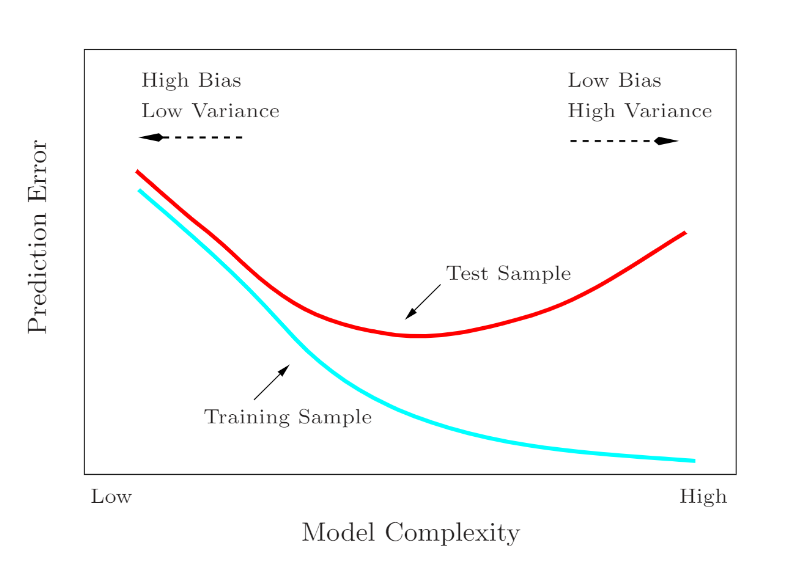
\includegraphics[width=0.9\textwidth]{figures/bias.PNG}

\section{Cross Validation}

Cross Validation is one technique to ensure effciency of the model. As discussed before, the data at hand is split into 3 separate sets. 

\begin{itemize}
  \item The training data is fed to the model for it to learn and build a classifier based on the input.
  \item Another Held-out data set is used to frequently test the performance of the model. Cross validation mainly deals with how data is split into training and validation datasets for better model verification.
  \item The testing dataset is used to provide the final model accuracy on a totally new data. This becomes a good estimate for the model's performance
\end{itemize}

One way achieve this is to randomly split data into 3 separate dataset and used them for training, validation and testing respectively. One backdraw in this technique is when there's very little data. It is important to have sufficient data at hand to train the model and equal important to have data for validation.

\subsection{K-fold cross validation}

One technique to follow is the \text{K-fold Cross Validation}. In this approach, we split the data into k sets, choose k-1 sets for training and 1 set for validations, then measure the error in prediction. Repeat this process k times with each of the k sets serving as a validation dataset once. Take average of these errors and choose the model with the least average validation error. +

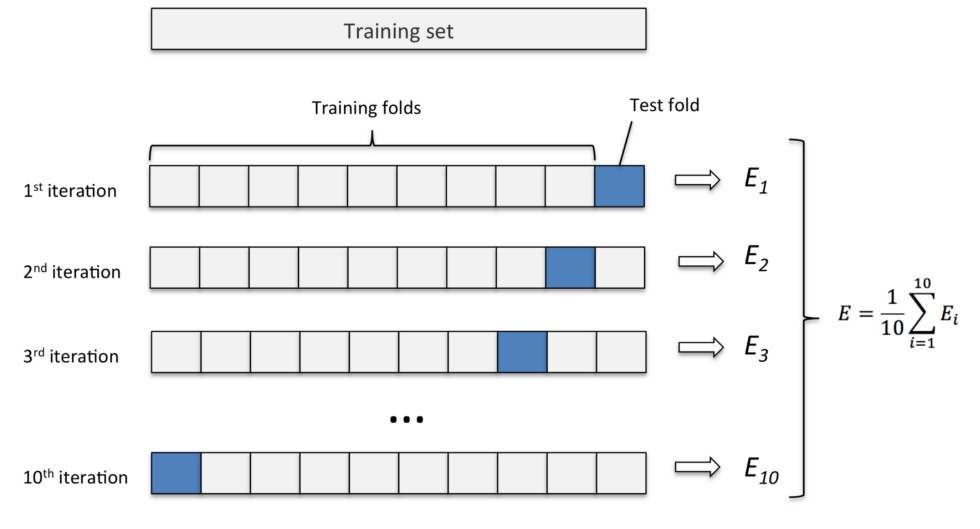
\includegraphics[width=0.8\textwidth]{figures/kfold.PNG}

\text{source: https://medium.com/@sebastiannorena/some-model-tuning-methods-bfef3e6544f0}

\section{Regularization}

Regularization is a way to penalize model complexity to allow it to generalize well to the future. One way to achieve this is to shrink the weights. The loss function is as given below.

\begin{equation}
    L = \frac{1}{n}\sum_{i=1}^{n}(y_i - wx_i)^2 + \lambda||w||^2
\end{equation}

here, as the $\lambda$ value increases the coefficient decreases. Thus, the weights are brought down for the model to generalize well



